%*************************************************************
% Preamble.
%*************************************************************
%*************************************************************
% Define the document properties.
%*************************************************************
\documentclass[12pt, letterpaper]{article}
\usepackage[hmargin=1in,vmargin=1in]{geometry}

%*************************************************************
% Restrict floats to the section in which they are defined.
%*************************************************************
\usepackage[section]{placeins}

%*************************************************************
% Appendix rules.
%*************************************************************

%*************************************************************
% Enumerated lists.
%*************************************************************
\usepackage{paralist}

%*************************************************************
% Make quotations display properly.
% Usage: \enquote{Stuff in quotes goes here.}
%*************************************************************
\usepackage{csquotes}

%*************************************************************
% Graphics and visuals.
%*************************************************************
\usepackage{graphicx}
\usepackage{subfig}
\usepackage{tabularx}

%*************************************************************
% Math packages.
%*************************************************************
\usepackage{amsmath}
%\usepackage{mathtools}																		% En­hance the ap­pear­ance of doc­u­ments con­tain­ing a lot of math­e­mat­ics.
%\usepackage{mathrsfs}																			% Other mathematical symbols.

%*************************************************************
% Astronomical symbols.
%*************************************************************
\usepackage{mathabx}
%\usepackage{marvosym} 																		% Maybe you don't have these packages instealled?
%\usepackage{wasysym}

%*************************************************************
% Make vectors look better.
%*************************************************************
\let\oldhat\hat
\renewcommand{\vec}[1]{\mathbf{#1}}
\renewcommand{\hat}[1]{\oldhat{\mathbf{#1}}}

%*************************************************************
% Bibliography related.
%*************************************************************
\usepackage{natbib}
\bibpunct{[} {]} {;} {a} {,} {,} 																		% Selecting citation style and punctuation.
%\usepackage[nottoc,numbib]{tocbibind} 													% Force citations page to appear in the T.O.C.

%*************************************************************
% For coloring citations/links and creating links.
%*************************************************************
\usepackage{hyperref}
\hypersetup{
  colorlinks=false,
  citecolor=purple,
  linkcolor=purple,
  urlcolor=purple}

%*************************************************************
% For text highlighting various colors.
%*************************************************************
\usepackage{soul}
\usepackage{color}
\usepackage[usenames,dvipsnames]{xcolor}
\newcommand{\hlc}[2][yellow]{ {\sethlcolor{#1} \hl{#2}} }

%*************************************************************
% Allow for adjustment of spacing on titles and headers.
%*************************************************************
\usepackage{titlesec}

%*************************************************************
% Change the font size of the section titles.
%*************************************************************
\titleformat*{\section}{\normalsize\bfseries\color{RoyalBlue}}
\titleformat*{\subsection}{\normalsize\bfseries\color{RoyalBlue}}
\titleformat*{\subsubsection}{\normalsize\bfseries\color{RoyalBlue}}
\titleformat*{\paragraph}{\normalsize\bfseries\color{RoyalBlue}}
\titleformat*{\subparagraph}{\normalsize\bfseries\color{RoyalBlue}}

%*************************************************************
% Begin the document.
%*************************************************************
\begin{document}

%*************************************************************
% Create the title.
%*************************************************************
%\noindent \normalsize{\color{RoyalBlue}{\bf{February 28, 2014}}} \\[0.125cm]
%\noindent \normalsize{\color{RoyalBlue}{\bf{To: Mike Liemohn}}} \\[0.125cm]
%\noindent \normalsize{\color{RoyalBlue}{\bf{From: Jonathan Nickerson}}} \\[0.125cm]
%\noindent \normalsize{\color{RoyalBlue}{\bf{RE: Modeling Study \#1}}} \\

%*************************************************************
% Create the title.
%*************************************************************
\noindent \large{\color{RoyalBlue}{\bf{Modeling Study \#2: An Empirical Description of Earth's Magnetopause Shape and Location for Real-Time Prediction of Magnetopause Crossings}}} \\[0.0cm]
\begin{center}
\normalsize{Jonathan S. Nickerson} \\[0.25cm]
\normalsize{March 23, 2014} \\[1cm]
\end{center}

%*************************************************************
% Begin a new section.
%*************************************************************
\section{Introduction}
\label{sec:introduction}
Earth has an intrinsic dipole magnetic field emanating from it's core which acts as an obstacle to the flow of the solar wind. The volume of space shielded from the solar wind is called the Earth's \emph{magnetosphere}. As the solar wind approaches Earth's magnetosphere, the flow of the solar wind must slow down in order to be diverted around the magnetospheric obstacle. Because this flow is highly supersonic and superalfv\'{e}nic ($M_{s} = \frac{u_{sw}}{a_{s}} \gtrsim 8$ and $M_{A} = \frac{u_{sw}}{v_{A}} \gtrsim 8$), a strong standing oblique shock wave forms upstream of the magnetosphere. This shock wave is called the \emph{bow shock} (because it resembles the wake created in front of a ships bow). The flow downstream of any oblique shock wave will always turn slightly toward the shock. This is because while the normal component of velocity always decreases across the shock, the tangential component will be conserved. Presumably this behavior consequently aids in redirecting the flow around the obstacle. None the less, the shocked solar wind will continue to flow subsonically toward the Earth's magnetosphere in a region known as the \emph{magnetosheath}. The boundary surface beyond which the shocked solar wind material cannot penetrate is called the \emph{magnetopause}. This is the point at which the solar wind thermal pressure inside of the magnetosheath ($P_{\text{magnetosheath}} = 0.85 \rho _{sw} u^{2}_{sw} \cos ^{2} \phi$) exactly balances the magnetic pressure from Earth's magnetosphere ($P_{B_{\Earth}} = \frac{B^{2}_{\Earth}}{2 \mu _{0}}$) \citep{Cravens97}. Here $\phi$ represents the angle between the direction of the solar wind flow and the normal to the magnetopause. Once inside the magnetosphere, the average densities are lower than those found in the solar wind. In the solar wind, charged particles are flowing away from the sun, along with the interplanetary magnetic field (IMF). Inside of the magnetosphere charged particles are instead guided along Earth's dipole field lines. In contrast to the compressed magnetosphere upwind from the Earth, down wind the dipole field gets stretched far downstream along with the solar wind, giving rise to a \emph{magnetotail}. The global shape and steady state behavior of the magnetosphere is thus analogous to the shape of a paraboloid with the vertex located at the sun-facing subsolar point.

The above discussion is a good starting point for understanding the magnetospause standoff distance. Several empirical models have been proposed to more accurately describe the general shape of the magnetopause as a function of solar wind dynamic pressure, $P_{\text{dyn}}$, and the IMF z-component, $B_{z}$ \citep{Petrinec93} \citep{Shue97} \citep{Shue98} \citep{Kuznetsov98} \citep{Roelof98}. Studies have shown that the \citet {Shue98} model has been the most successful at describing the shape of the magnetopause \citep{Shue00}. For this reason I used this model for my study. 

%*************************************************************
% Begin a new section.
%*************************************************************
\section{Summary of the Model}
\label{sec:summary} 
The model first proposed by \citet{Shue97} is given as 
\begin{equation}
r = r_{0} \left( \frac{2}{1 + \cos \theta } \right) ^{\alpha}
\end{equation}
where $r_{0}$ and $\alpha$ are the standoff distance and the level of tail flaring, respectively. These are defined as follows
\begin{equation}
 r_{0} =
  \begin{cases}
   \left( 11.4 + 0.013 B_{z} \right) P_{\text{dyn}}^{-\frac{1}{6.6}} & \text{for} B_{z} \vargeq 0 \\
   \left( 11.4 + 0.14 B_{z} \right) P_{\text{dyn}}^{-\frac{1}{6.6}} & \text{for} B_{z} < 0 
  \end{cases}
\end{equation}
\begin{equation}
\alpha = \left( 0.58 - 0.010 B_{z} \right) \left( 1 + 0.010 P_{\text{dyn}} \right ).
\end{equation}
Over the following year it was found that this model caused excess flaring in the magnetotail region for large values of $P_{\text{dyn}}$. Thus \citet{Shue98} proposed a correction to the model by changing $r_{0}$ and $\alpha$ to include a nonlinear dependence of the parameters on the solar wind conditions as follows
\begin{equation}
r_{0} = \lbrace 10.22 + 1.29 \tanh \left[ 0.184 \left( B_{z} + 8.14 \right) \right] \rbrace P_{\text{dyn}}^{-\frac{1}{6.6}}
\end{equation}
\begin{equation}
\alpha = \left( 0.58 - 0.007 B_{z} \right) \left[ 1 + 0.024 \log \left( P_{\text{dyn}} \right ) \right].
\end{equation}
In my study I used the \citet{Shue98} revised model. To understand the model response to upstream solar wind conditions I did a sensitivity study. I then proceeded with a data-model comparison to test the model's ability to predict magnetopause crossings of the GOES 10 satellite. 

%*************************************************************
% Begin a new section.
%*************************************************************
\section{Sensitivity Study}
\label{sec:sensitivity}
\subsection{Methodology}
The Shue model relies on only two input parameters, $P_{\text{dyn}}$ and $B_{z}$. To characterize the general behavior of the model I investigated how the model responds to both of these parameters. To do accomplish this I varied one of the parameters while holding the other constant, and vice versa. 

\subsection{Results}
\textcolor{RoyalBlue}{Figure \ref{fig:sens_magnetopause}} (\textcolor{RoyalBlue}{Appendix \ref{sec:B}}) shows the cross section of the magnetopause demonstrating shape and location sensitivity to $B_{z}$ while holding $P_{\text{dyn}}$ constant and vice versa. We can see that a southward IMF pushes the magnetopause inward and causes the tail to flare. As $B_{z}$ becomes more negative, the pushing and flaring become more dramatic. In contrast, a northward IMF causes pinching of the tail with increasing strength but does little to push the magnetopause inward. Increasing solar wind pressure pushes the magnetopause inward without flaring or pinching. I would like to note that by increasing $P_{\text{dyn}}$ to unreasonably large values, the magnetopause continues to push inward until it no longer represents a configuration that we would expect to find in reality. In this extreme case the shape of $r$ becomes that of an ellipsoid that eventually vanishes inside of 1 R$_{\Earth}$. The affect that $B_{z}$ has on the magnetopause location for a range of $P_{\text{dyn}}$ is summed up in \textcolor{RoyalBlue}{Figure \ref{fig:sens}}. Plotting $r$ as a function of $B_{z}$. Varying $P_{\text{dyn}}$ from $9 \left[ \text{nPa} \right]$ to $34 \left[ \text{nPa} \right]$ in even intervals. We see the effect that a southward IMF has on pushing the magnetopause inside of geosynchronous orbit (denoted by the dotted line) for a given $P_{\text{dyn}}$. In a similar approach, varying $B_{z}$ from $-60 \left[ nT \right]$ to $60 \left[ nT \right]$ in 50 evenly spaced increments we see the range of $P_{\text{dyn}}$ required for a given value of $B_{z}$ to push the magnetopause inside of geosynchronous orbit. 

%*************************************************************
% Begin a new section.
%*************************************************************
\section{Data-Model Comparison}
\label{sec:data-model}
\subsection{Methodology}
It is commonly believed that one advantage to empirical models is that because they are computationally inexpensive and quick to calculate they are ideal for real time forecasting. A primary goal of this study is to determine if this model can be used in conjunction with upstream solar wind conditions measured by the Advanced Composition Explorer (ACE) spacecraft to reliably predict real-time magnetopause crossings for the Geostationary Satellite System (GOES) 10 satellite. 

The ACE spacecraft is located at the L2 Lagrange point ($\sim 235 R_{\Earth}$ upstream). At typical solar wind speeds it takes about an hour for the solar wind to propagate to the Earth from ACE's position. Solar wind ACE data has been processed and prepropagated and made available online at OMNIWeb, which is hosted by NASA. I obtained the input data for my study here.

GOES 10 sits in geosynchronous orbit at $\sim 6.6 R_{\Earth}$. Under adequately strong upstream solar wind conditions the magnetopause can be pushed inside of $\sim 6.6 R_{\Earth}$. When this happens, provided GOES 10 is on the day side of Earth, GOES 10 will experience a magnetopause crossing. A crossing will manifest itself in the GOES 10 $B_{z}$ magnetometer measurement as an abrupt reversal of the $B_{z}$ magnetic field from strongly positive to strongly negative (\textcolor{RoyalBlue}{Figure \ref{fig:GOES_Bz}}). GOES 10 data for this study was obtained from CDAWeb, also hosted by NASA. 

GOES 10 measured magnetopause crossings on the following five dates: 
\begin{inparaenum}[$\cdot$]
  \item Sep 23, 1999
  \item Apr 07, 2000
  \item Sep 18, 2000
  \item Mar 31, 2001
  \item Apr 12, 2001.
\end{inparaenum} 
I compared the models cumulative predictive capabilities ranging over these five events. For each of the events I took a 10-minute running average (\textcolor{RoyalBlue}{Figure \ref{fig:GOES_Bz}}). This allowed for cleaning up the signal to separate the noise/fluctuations from the physically meaningful data.

\subsection{Results}
The result of the data-model comparison can be visualized in \textcolor{RoyalBlue}{Figure \ref{fig:movie}}. Looking down from the north pole of the Earth, we can see the position of GOES 10 as it orbits the Earth projected into the x-y plane. The predicted position of the magnetopause is also shown. Through the sequence we can see a predicted magnetopause crossing. For a more thorough visualization of the result please follow the link to a movie of the sequence. While the result looks pretty good, it isn't meaningful without comparing the predicted crossings to the model to the actual measurement taken by GOES 10.

\subsection{Analysis}
The best way to analyze the quality of a predictive model of this kind is to build a \emph{contingency table}. The contingency table allows for comparison of the state of the model to the state of the data. Because the data was \enquote{binned} into 10 minute intervals, each of the five events had a total of 288 frames. The contingency table, shown in \textcolor{RoyalBlue}{Appendix \ref{sec:A}}, is for all five events combined. A \enquote{hit}, denoted as (H), is when the model and the data both indicate that the satellite is outside of the magnetopause. A \enquote{miss}, denoted as (M), is when the data shows that GOES 10 is outside of the magnetopause but the model thinks it should be inside. A \enquote{false alarm}, denoted as (F), indicates when the data shows the satellite inside of the magnetopause and the data shows it outside. Lastly a \enquote{correct negative}, denoted as (N), is when both the data and the model indicate that the satellite should be inside of the magnetopause. The corresponding values are the number of times each of these criteria were met across all five events. Because the satellite spends most of its time inside the magnetopause in the dusk, midnight, and dawn sectors we would expect N to be the largest value. 

The contingency table allows us to do some basic statistical analysis to get a feel for how \enquote{good} the model is. We can calculate the probability of detection (POD), which is the probability that the model will detect a correct magnetopause crossing as follows
\begin{eqnarray}
\text{POD} & = & \frac{\text{H}}{\text{H} + \text{M}} \nonumber \\
& & \nonumber \\
& = & 49.52 \%
\end{eqnarray}
For this study I found $\text{POD} = 49.52\%$. This may seem low but I think it is pretty good considering the many factors that could fudge the result. I think that for any predictive model, this is the range one might could expect. One thing that lowered this score is that while the model predicted that there would be a crossing every time that one happened, it did not predict all events during the time interval in which they actually happened. There was no specific pattern to the offsetting of the models predictive capability. If so we might expect that we could time-shift our input data to better match the result (for example if there is a lag in the propagation of ACE data). Perhaps for this model, a 10-minute running average might be too small of a bin size. Increasing the bin size would definitely drive up its apparent predictive capabilities, but one must tread carefully here. Doing so might very well wash out the usefulness of the model. 

Next we can look at the probability of false detection as follows
\begin{eqnarray}
\text{POFD} & = & \frac{\text{F}}{\text{F} + \text{N}} \nonumber \\
& & \nonumber \\
& = & 0.90 \%
\end{eqnarray}
I found $\text{POFD} = 0.90\%$. This value is very low which is a good thing. The model does a good job at keeping the false detection to a minimum.

Lastly we can look at the Heidke skill score (skill score for short). The HSS is given as
\begin{eqnarray}
\text{HSS} & = & \frac{2 \left[ \left( \text{H} \cdot \text{N} \right) - \left( \text{M} \cdot \text{F} \right) \right]}{\left( \text{H} + \text{M} \right) \left( \text{M} + \text{N} \right) + \left( \text{H} + \text{F} \right) \left( \text{F} + \text{N} \right)} \nonumber \\
& & \nonumber \\
& = & 0.593
\end{eqnarray}
For this model we find that $\text{HSS} = 0.593$. This is a pretty decent value. A perfect score is a 1.0. Such a score would be the Holy Grail of predictive models. In reality most models are less than 1.0. A skill score with a negative value basically indicates that the models predictive capabilities are worse than not having a model at all. Realistically, any forecasting model with a value above 0.50 is considered good.

%*************************************************************
% Begin a new section.
%*************************************************************
\section{Summary}
\label{sec:6}
In this study I investigated the quality of the empirical model proposed by \citep{Shue98}. I first began with a sensitivity study to understand how the model behaved as a function of its input parameters, $P_{\text{dyn}}$ and IMF $B_{z}$. I found that a large southward IMF will drive the model's description of the magnetopause location inward and flare the tail. In contrast a large northward IMF will not compress the magnetopause location, however rather than flaring the tail it instead pinches it. Increasing the solar wind pressure has the result of only compressing the magnetopause while not causing any flaring or pinching. Next, I investigated the models predictive capabilities. I used prepropagated ACE data as the input values to the model. I compared the resulting predicted magnetopause locations to the location of the GOES 10 spacecraft. I looked at the GOES 10 magnetometer data to see when it actually detected a magnetopause crossing and compared that to when the model predicted that a crossing should happen. I was able to characterize five events in total. Using a contingency table I was able to calculate the probability of detection to be $\text{POD} = 49.52\%$, the probability of false detection of $\text{POFD} = 0.90\%$ and a skill score value of $\text{HSS} = 0.593$. In conclusion this model seems to do a pretty good job overall at predicting that a magnetopause corssing \emph{will} occur. Its shortcoming is in the time resolution. It does not do a good job at predicting \emph{when} a crossing will occur. In other words, even though the model nearly always indicates that an even will happen, it does not happen within the same $\Delta t$ as the actual measurement. The model was often between 30 minutes to 3 hours off. This calls in to question how useful the model will be for applications in which needing to know the chance of an event on time scales of less than 3 hours are important.

%*************************************************************
% Begin Appendix.
%*************************************************************
\appendix
%*************************************************************
% Begin a new section.
%*************************************************************
\newpage
\section{Tables}
\label{sec:A}
\renewcommand{\arraystretch}{1.5}
\begin{table}[!ht]
\centering
\caption{Contingency Table.}
\begin{tabular}{| l | c | c | c |} % Using the p column descriptor to allow for text wrapping in my table.
\hline
\rule{0pt}{4.5mm}
 & Model: Outside Magnetopause & Model: Inside Magnetopause \\
\hline
Data: Outside Magnetopause & H: 52 & M: 53 \\
\hline
Data: Inside Magnetopause & F: 12 & N: 1323 \\
\hline
\end{tabular}
\label{table:1}
\end{table}

%*************************************************************
% Begin a new section.
%*************************************************************
\newpage
\section{Figures}
\label{sec:B}
\begin{figure}
\def\tabularxcolumn#1{m{#1}}
\begin{tabularx}{\linewidth}{@{}cXX@{}}
\begin{tabular}{cc}
\subfloat[]{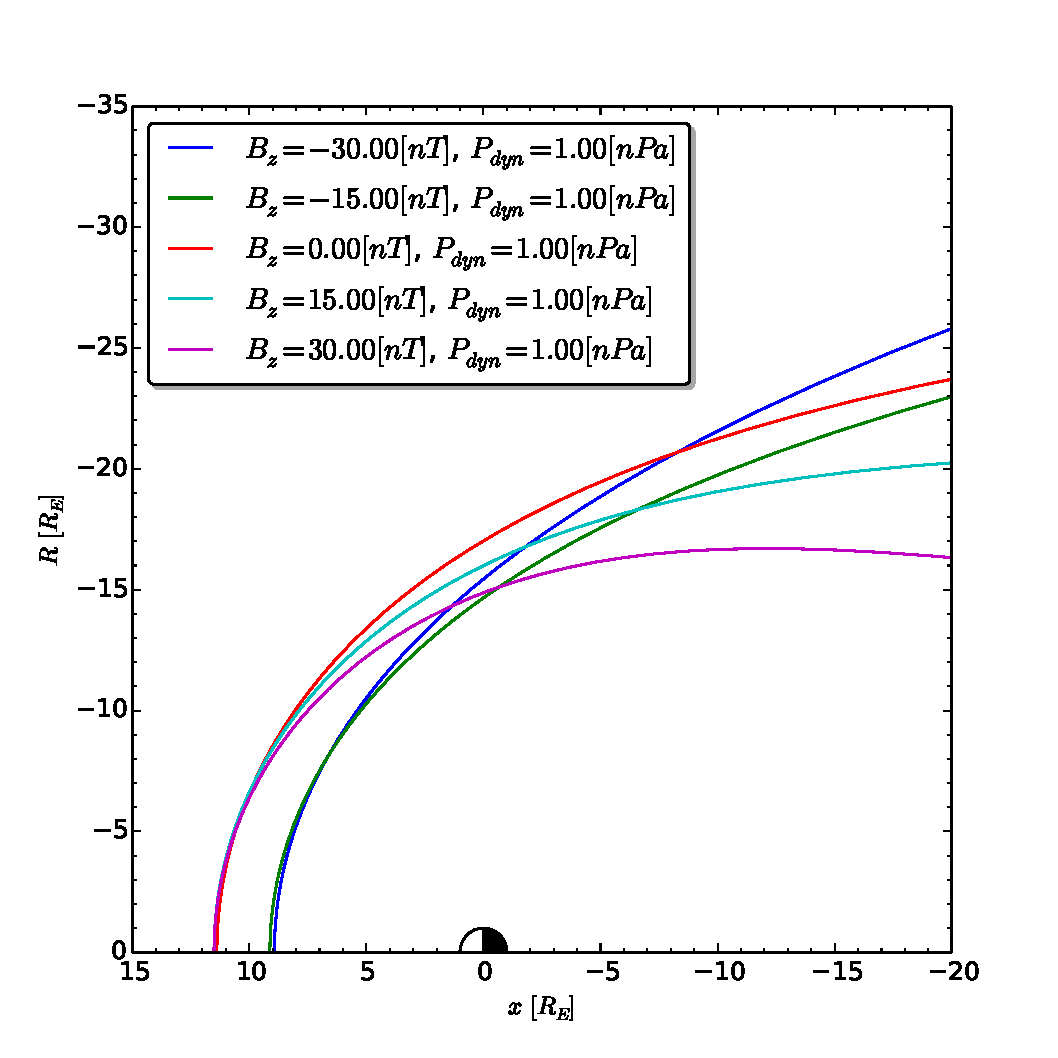
\includegraphics[width=0.49\textwidth]{./plots_&_images/sensitivity_study/dBz.pdf}}
   & \subfloat[]{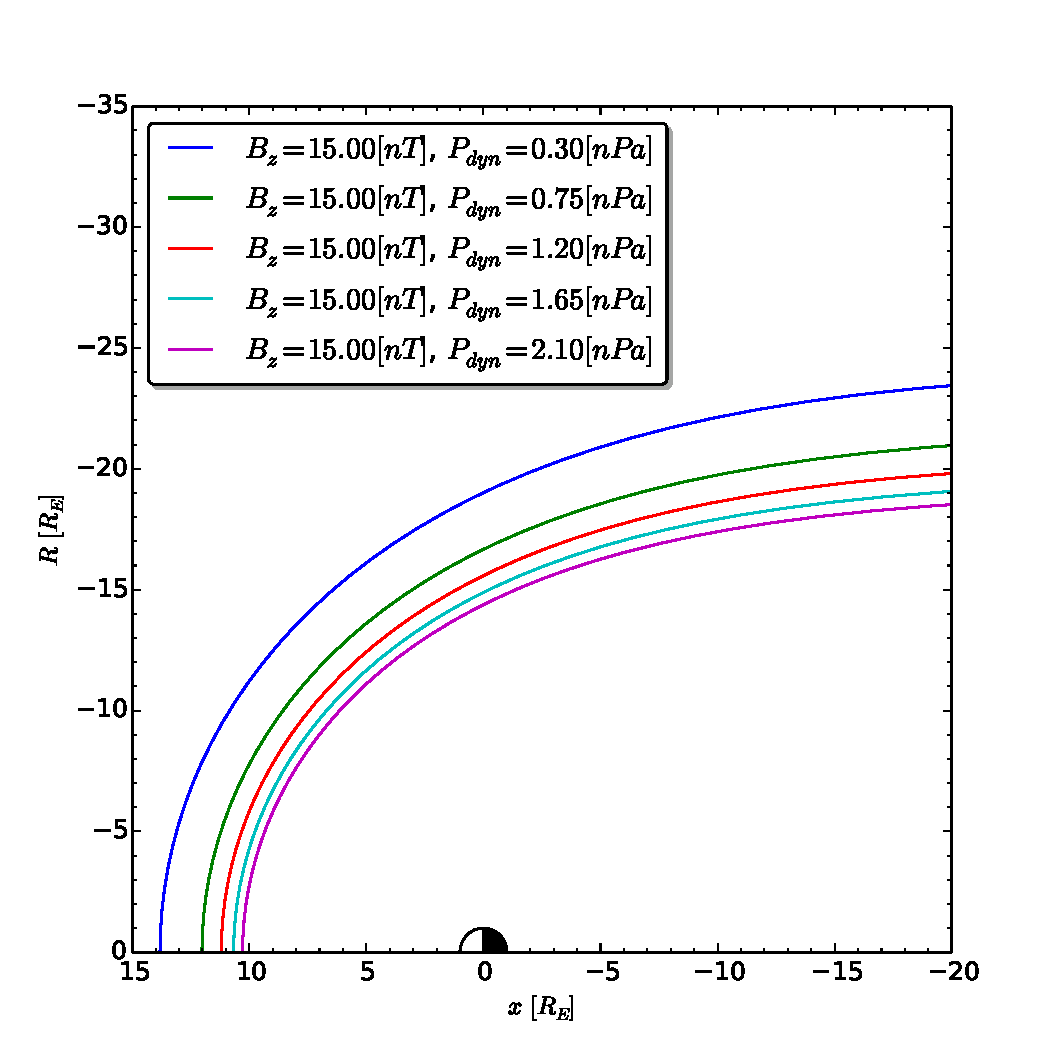
\includegraphics[width=0.49\textwidth]{./plots_&_images/sensitivity_study/dDp.pdf}}\\
\end{tabular}
\end{tabularx}
\caption{a) Magnetopause location sensitivity to $B_{z}$. We see that a southward IMF pushes the magnetopause inward as well as causing the tail to flare. In contrast a northward IMF does not push the magnetopause inward but does cause pinching of the tail. b) Magnetopause location sensitivity to $P_{\text{dyn}}$. Clearly $P_{\text{dyn}}$ has no effect on flaring or pinching but does compress the entire magnetopause inward.}
\label{fig:sens_magnetopause}
\end{figure}

\begin{figure}
\def\tabularxcolumn#1{m{#1}}
\begin{tabularx}{\linewidth}{@{}cXX@{}}
\begin{tabular}{cc}
\subfloat[]{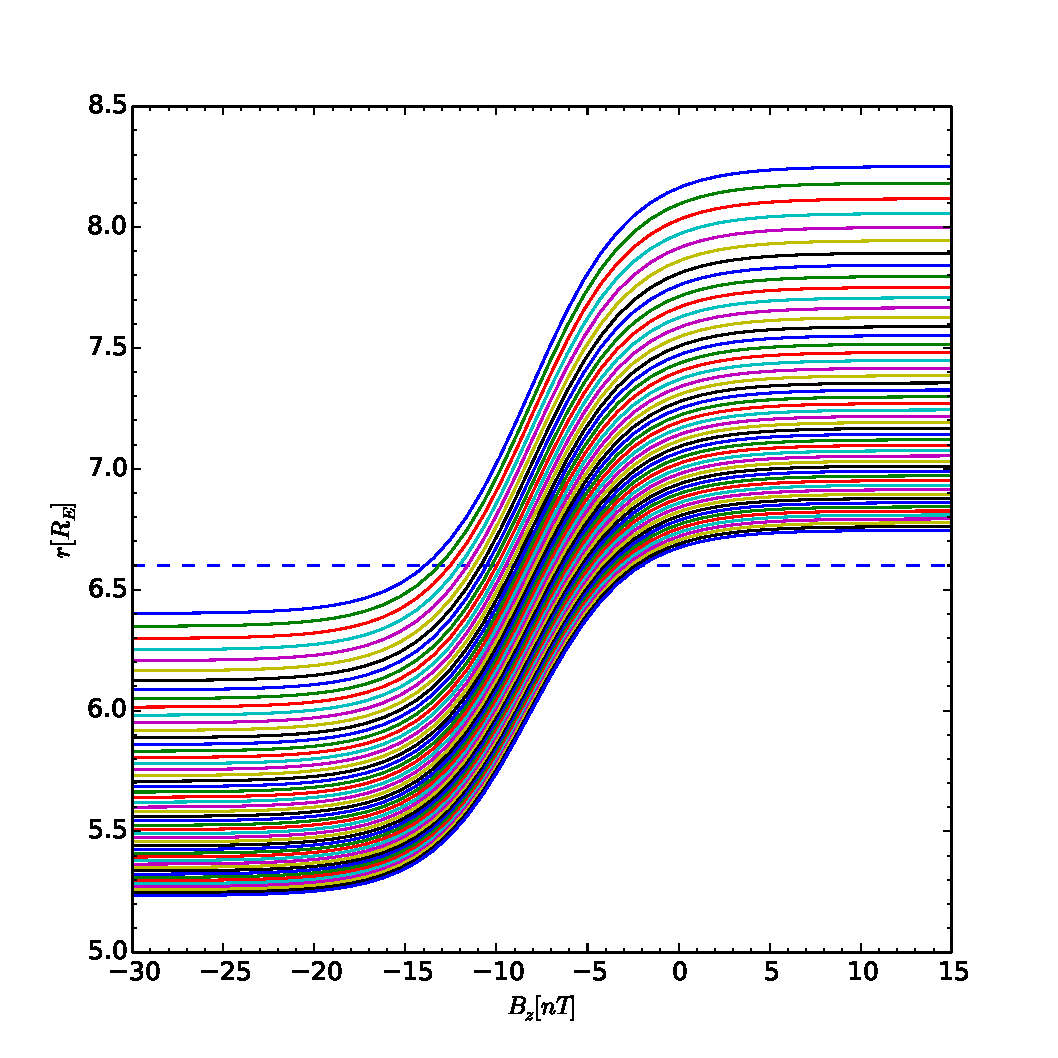
\includegraphics[width=0.49\textwidth]{./plots_&_images/sensitivity_study/rvsBz.pdf}}
   & \subfloat[]{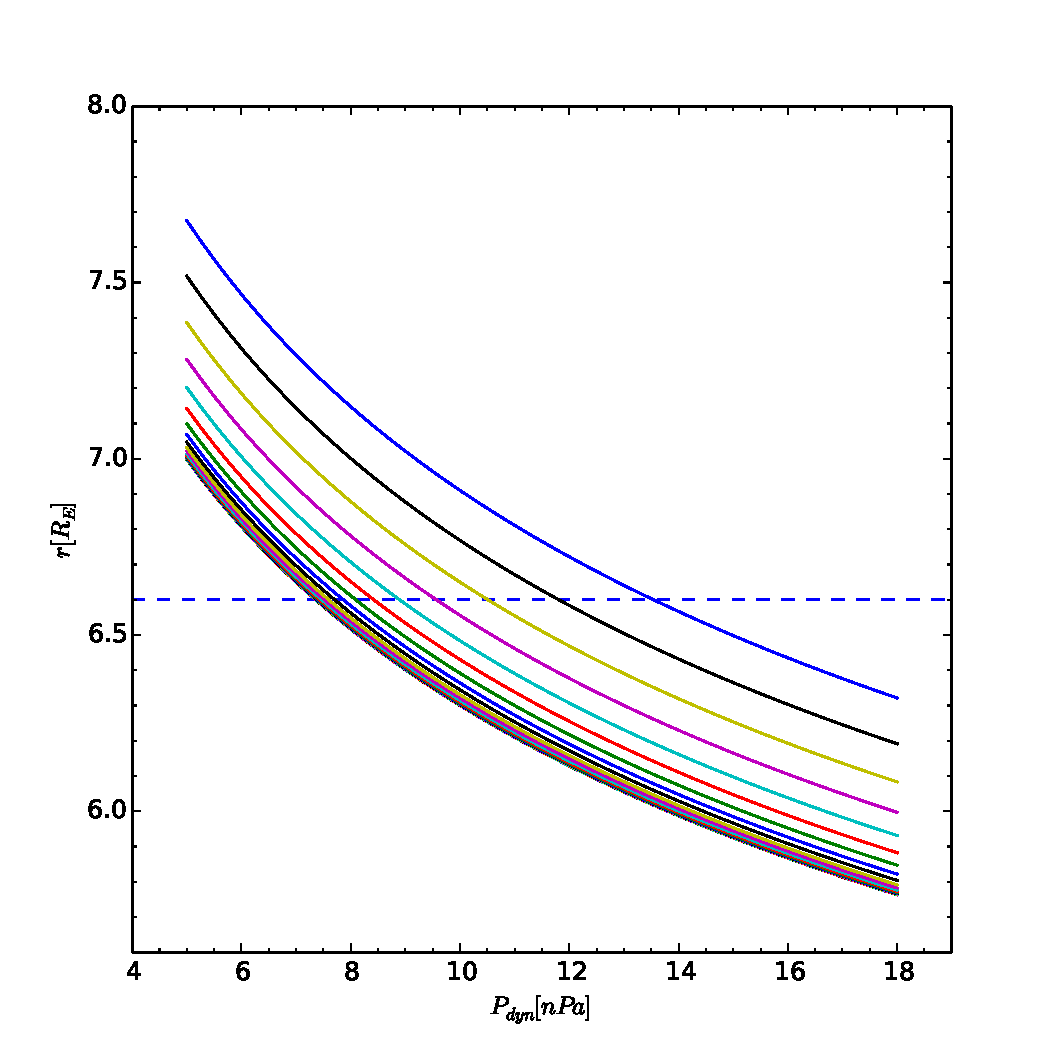
\includegraphics[width=0.49\textwidth]{./plots_&_images/sensitivity_study/rvsDp.pdf}}\\
\end{tabular}
\end{tabularx}
\caption{a) Plotting $r$ as a function of $B_{z}$. Varying $P_{\text{dyn}}$ from $9 \left[ \text{nPa} \right]$ to $34 \left[ \text{nPa} \right]$ in even intervals. We see the effect that a southward IMF has on pushing the magnetopause inside of geosynchronous orbit (denoted by the dotted line) for a given $P_{\text{dyn}}$. b) In a similar approach, varying $B_{z}$ from $-60 \left[ nT \right]$ to $60 \left[ nT \right]$ in 50 evenly spaced increments we see the range of $P_{\text{dyn}}$ required for a given value of $B_{z}$ to push the magnetopause inside of geosynchronous orbit.}
\label{fig:sens}
\end{figure}

\begin{figure}
\def\tabularxcolumn#1{m{#1}}
\begin{tabularx}{\linewidth}{@{}cXX@{}}
\begin{tabular}{cc}
\subfloat[]{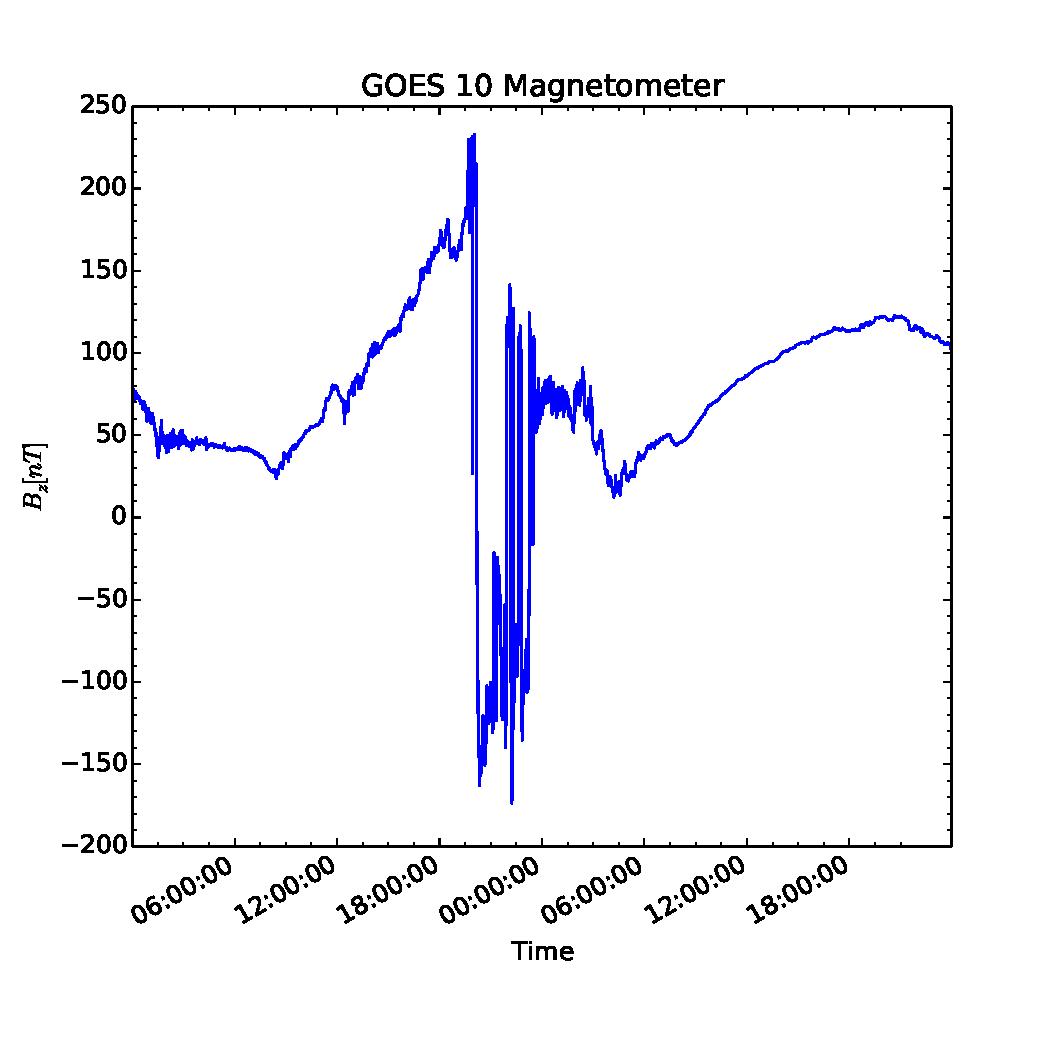
\includegraphics[width=0.49\textwidth]{./plots_&_images/data-model_comparison/GOES_BzvsTime_raw.pdf}}
   & \subfloat[]{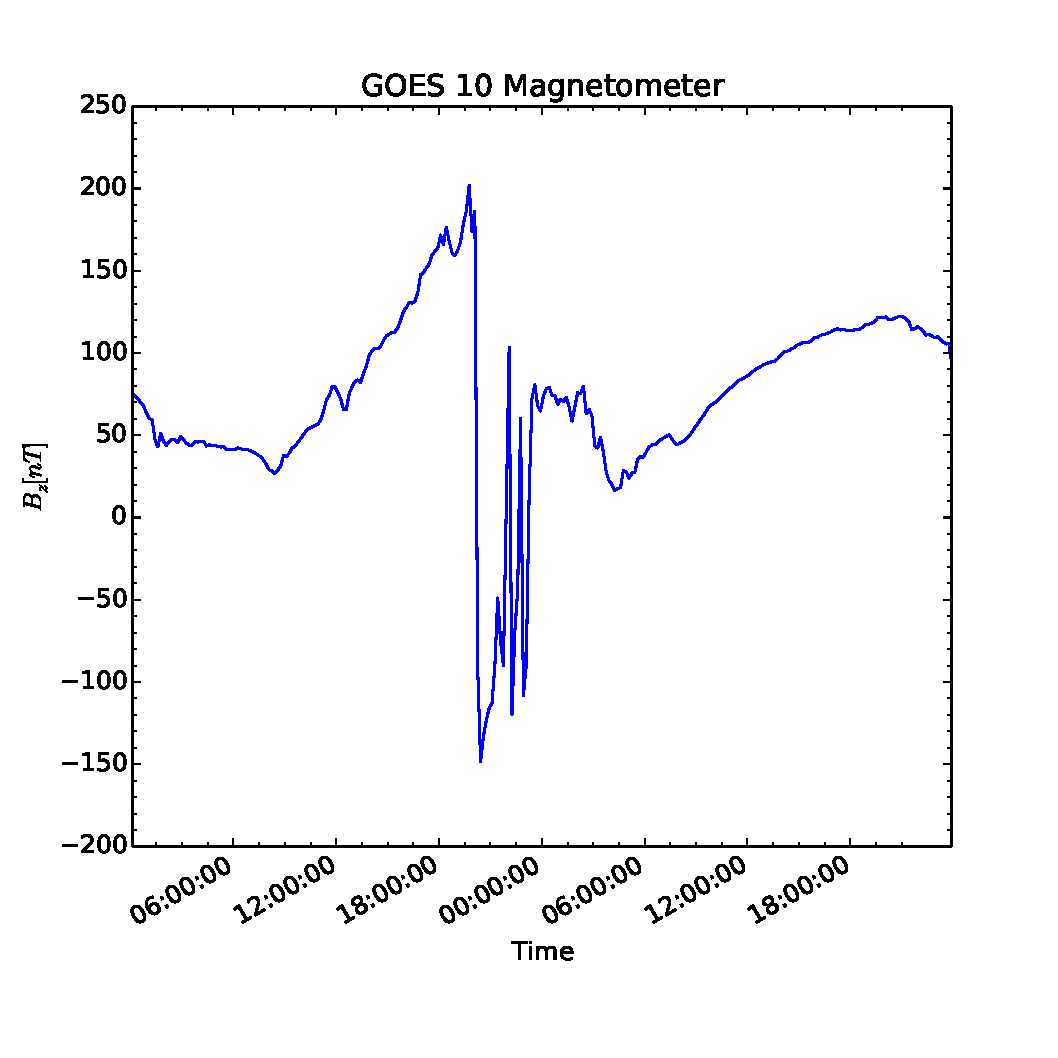
\includegraphics[width=0.49\textwidth]{./plots_&_images/data-model_comparison/GOES_BzvsTime.pdf}}\\
\end{tabular}
\end{tabularx}
\caption{a) Plotting GOES $B_{z}$ magnetometer data vs Time for the event of Sep 23, 1999. For a crossing we expect a strong northward $B_{z}$ component followed by a sudden reversal to a strong southward $B_{z}$ component. Indeed this is precisely what we see. b) The same interval after taking a 10-minute running average of the signal. The data is cleaned up significantly separating the noise from the physically meaningful data.} 
\label{fig:GOES_Bz}
\end{figure}

\label{sec:B}
\begin{figure}
\def\tabularxcolumn#1{m{#1}}
\begin{tabularx}{\linewidth}{@{}cXX@{}}
\begin{tabular}{cc}
\subfloat[]{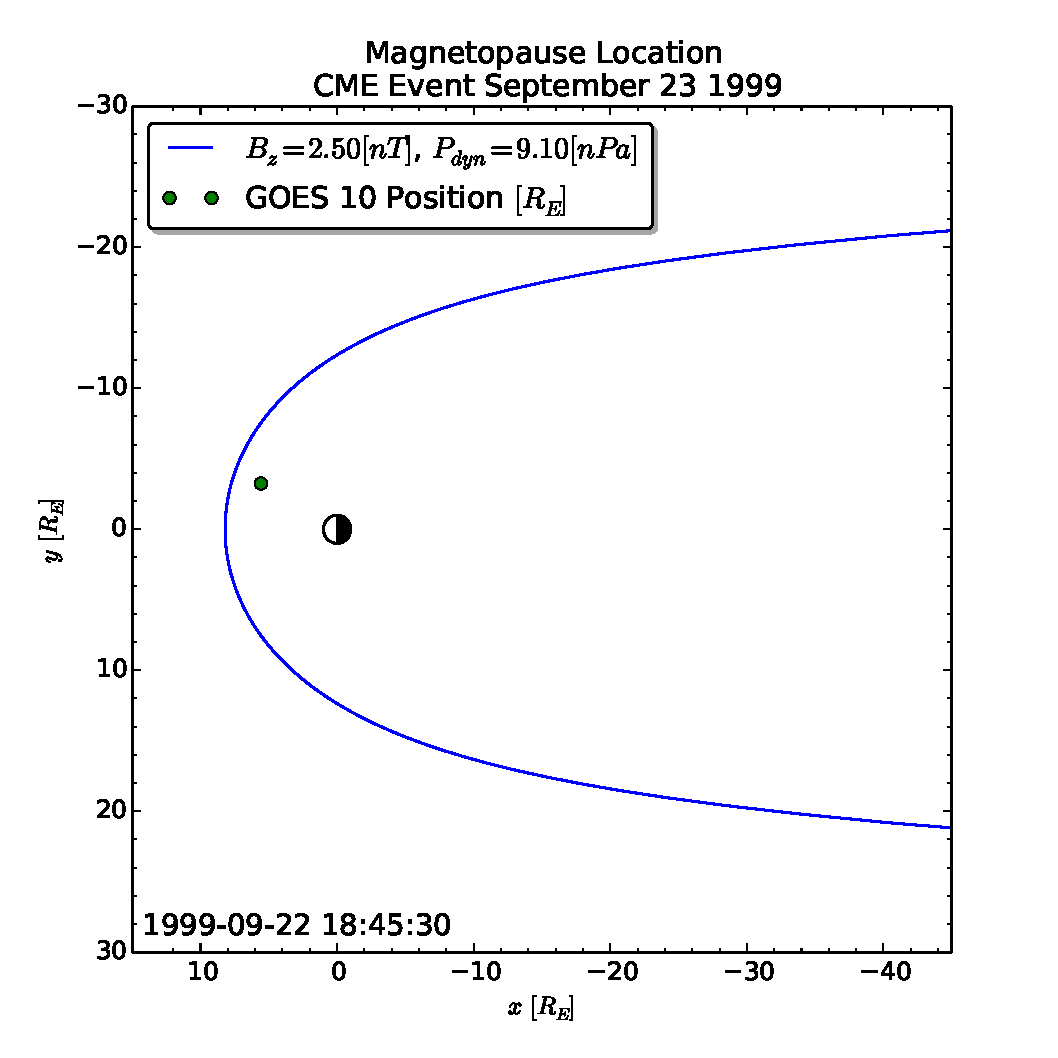
\includegraphics[width=0.49\textwidth]{./plots_&_images/data-model_comparison/112.pdf}} 
   & \subfloat[]{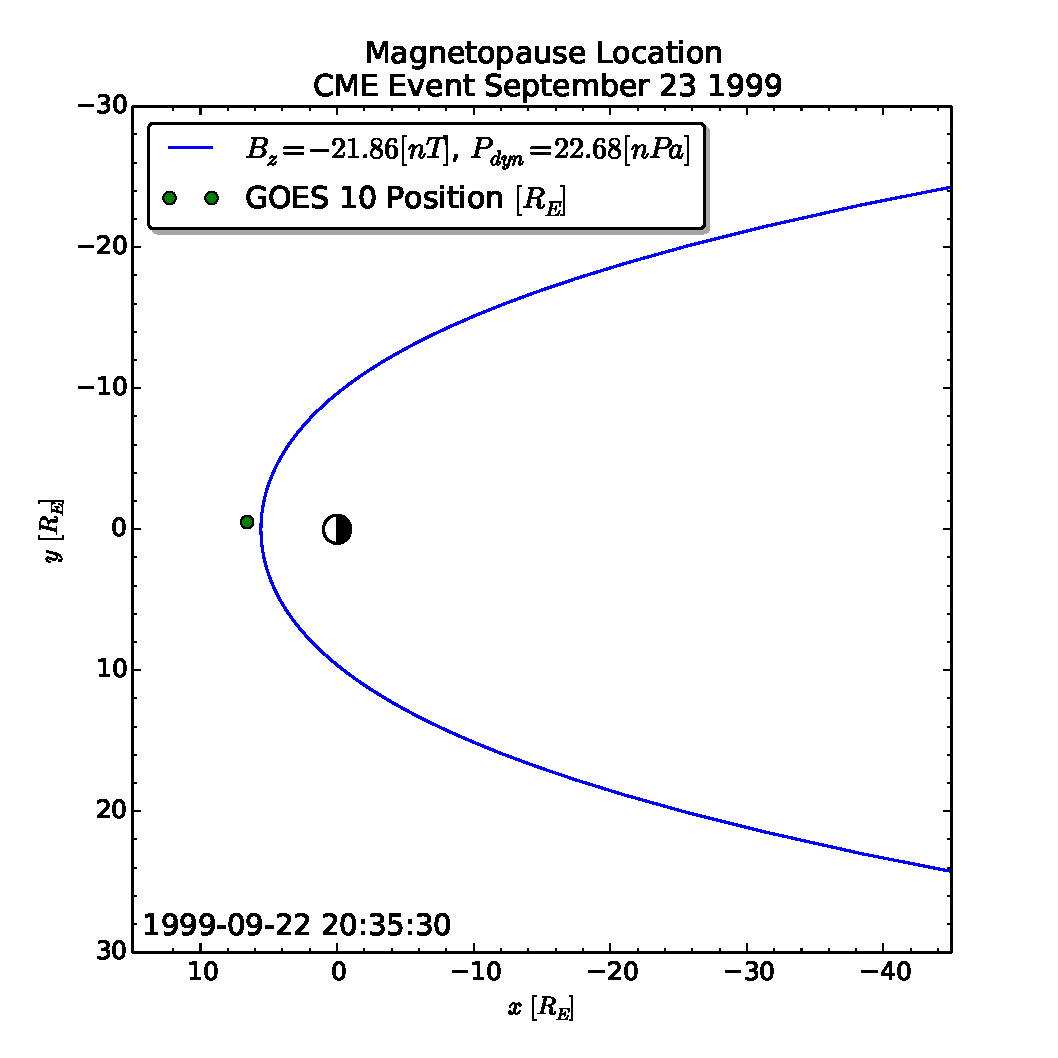
\includegraphics[width=0.49\textwidth]{./plots_&_images/data-model_comparison/123.pdf}}\\
\subfloat[]{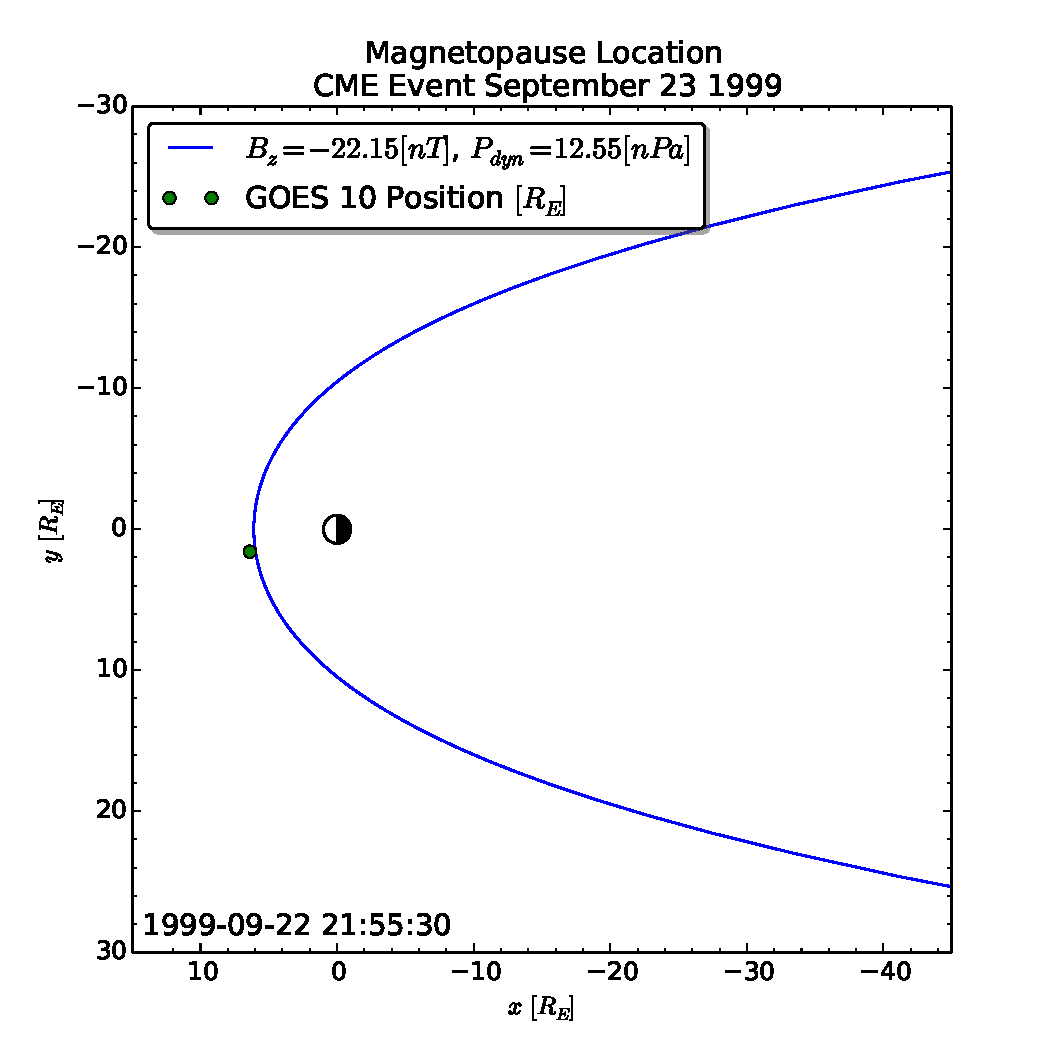
\includegraphics[width=0.49\textwidth]{./plots_&_images/data-model_comparison/131.pdf}} 
   & \subfloat[]{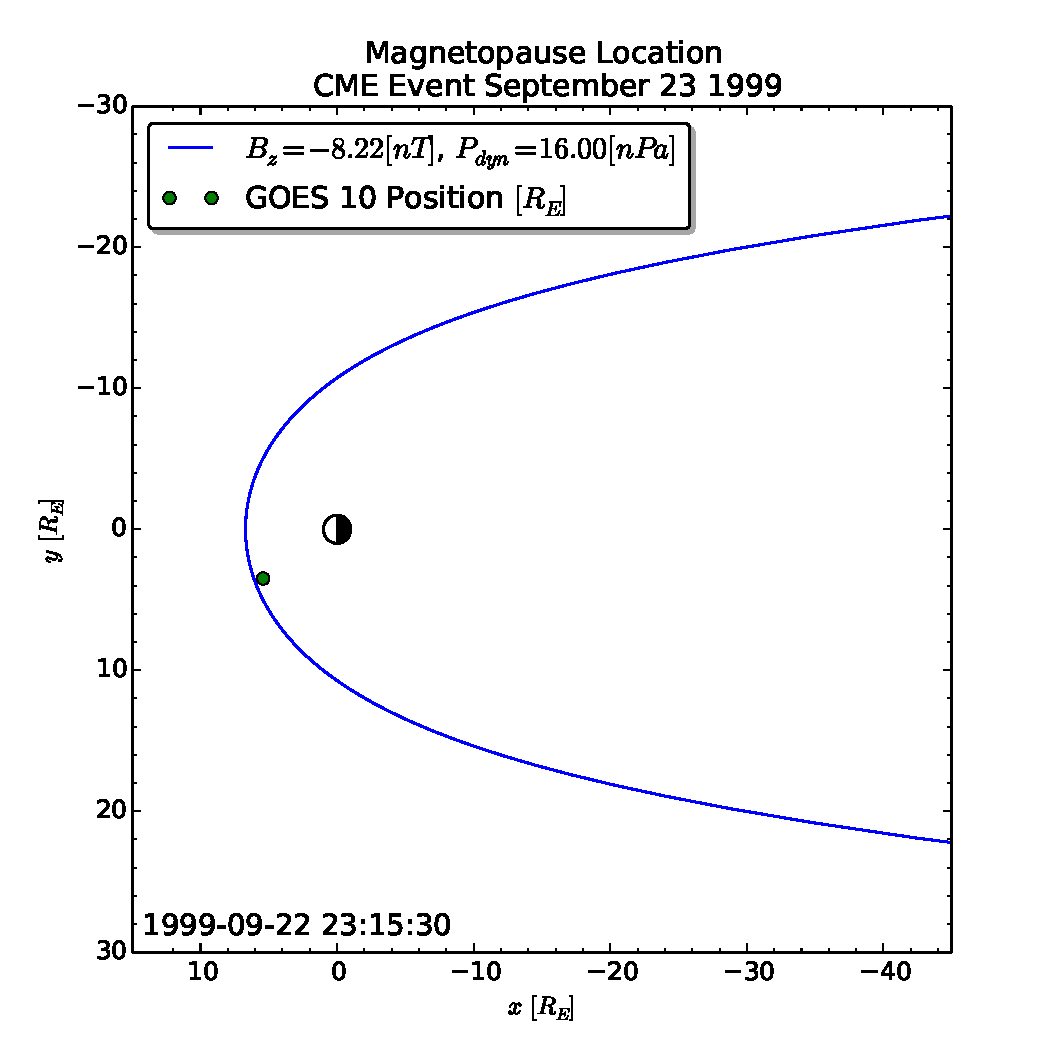
\includegraphics[width=0.49\textwidth]{./plots_&_images/data-model_comparison/139.pdf}}\\
\end{tabular}
\end{tabularx}
\caption{Plotting the position of GOES 10 relative to the predicted location of the magnetopause. We can see GOES 10 undergo a magnetopause crossing in this sequence. \color{RoyalBlue}{\href{https://dl.dropboxusercontent.com/u/52982963/Shue_movie.mov}{Click here for a movie of this sequence.}}}
\label{fig:movie}
\end{figure}

%*************************************************************
% Typset the bibliography
%*************************************************************
\newpage
\bibliographystyle{./bibliography/agu08} 														% AGU citation style sheet
\bibliography{./bibliography/bibliography}  													% Master bibliography list

%*************************************************************
% End the document environment.  
% No other lines will be read after this point.
%*************************************************************
\end{document}